\documentclass[]{article}
\usepackage[utf8]{inputenc}
\usepackage[spanish]{babel}
\usepackage{graphicx, graphics, float, fancyhdr, titling, caption, subcaption, amsmath}
\usepackage{listings,xcolor}
\usepackage[a4paper, total={6in, 9.5in}]{geometry}
\usepackage{fancyhdr}
\usepackage{hyperref}   %para que funcione addcontentsline debe ser la ultima que se cargue

\usepackage{blindtext}
\usepackage{mwe}

%\setcounter{secnumdepth}{-2}       %Poner solo esto si no se quieren numero delante de las secciones y niveles inferiores.

\renewcommand{\footrulewidth}{0.4pt}
\title{

\includegraphics[width=1.75in]{imagenes/UGR-Logo.png} \\
\vspace*{1in}
\textbf{Memoria de la Práctica 7} \\
Animación por Ordenador \\
\vspace*{0.5in}}
\author{Andrés Merlo Trujillo \\
andresmerlo@correo.ugr.es \\
77147239H \\ 
\vspace*{0.5in} \\
E.T.S. de Ingenierías Informática y de Telecomunicación \\
\textbf{Universidad de Granada}} \date{\today}

\hypersetup{
    colorlinks=true,
    linkcolor=black,
    citecolor=black
}

\renewcommand\maketitlehooka{\null\mbox{}\vfill}
\renewcommand\maketitlehookd{\vfill\null}

\definecolor{codegreen}{rgb}{0,0.6,0}
\definecolor{codegray}{rgb}{0.5,0.5,0.5}
\definecolor{codepurple}{rgb}{0.58,0,0.82}
\definecolor{backcolour}{rgb}{0.95,0.95,0.92}

\lstdefinestyle{mystyle}{
    backgroundcolor=\color{backcolour},   
    commentstyle=\color{codegreen},
    keywordstyle=\color{magenta},
    numberstyle=\tiny\color{codegray},
    stringstyle=\color{codepurple},
    basicstyle=\ttfamily\footnotesize,
    breakatwhitespace=false,         
    breaklines=true,                 
    captionpos=b,                    
    keepspaces=true,                 
    numbers=left,                    
    numbersep=5pt,                  
    showspaces=false,                
    showstringspaces=false,
    showtabs=false,                  
    tabsize=2,
    literate=
  {á}{{\'a}}1 {é}{{\'e}}1 {í}{{\'i}}1 {ó}{{\'o}}1 {ú}{{\'u}}1
  {Á}{{\'A}}1 {É}{{\'E}}1 {Í}{{\'I}}1 {Ó}{{\'O}}1 {Ú}{{\'U}}1
  {à}{{\`a}}1 {è}{{\`e}}1 {ì}{{\`i}}1 {ò}{{\`o}}1 {ù}{{\`u}}1
  {À}{{\`A}}1 {È}{{\`E}}1 {Ì}{{\`I}}1 {Ò}{{\`O}}1 {Ù}{{\`U}}1
  {ä}{{\"a}}1 {ë}{{\"e}}1 {ï}{{\"i}}1 {ö}{{\"o}}1 {ü}{{\"u}}1
  {Ä}{{\"A}}1 {Ë}{{\"E}}1 {Ï}{{\"I}}1 {Ö}{{\"O}}1 {Ü}{{\"U}}1
  {â}{{\^a}}1 {ê}{{\^e}}1 {î}{{\^i}}1 {ô}{{\^o}}1 {û}{{\^u}}1
  {Â}{{\^A}}1 {Ê}{{\^E}}1 {Î}{{\^I}}1 {Ô}{{\^O}}1 {Û}{{\^U}}1
  {ã}{{\~a}}1 {ẽ}{{\~e}}1 {ĩ}{{\~i}}1 {õ}{{\~o}}1 {ũ}{{\~u}}1
  {Ã}{{\~A}}1 {Ẽ}{{\~E}}1 {Ĩ}{{\~I}}1 {Õ}{{\~O}}1 {Ũ}{{\~U}}1
  {œ}{{\oe}}1 {Œ}{{\OE}}1 {æ}{{\ae}}1 {Æ}{{\AE}}1 {ß}{{\ss}}1
  {ű}{{\H{u}}}1 {Ű}{{\H{U}}}1 {ő}{{\H{o}}}1 {Ő}{{\H{O}}}1
  {ç}{{\c c}}1 {Ç}{{\c C}}1 {ø}{{\o}}1 {Ø}{{\O}}1 {å}{{\r a}}1 {Å}{{\r A}}1
  {€}{{\euro}}1 {£}{{\pounds}}1 {«}{{\guillemotleft}}1
  {»}{{\guillemotright}}1 {ñ}{{\~n}}1 {Ñ}{{\~N}}1 {¿}{{?`}}1 {¡}{{!`}}1,
  extendedchars=true
}

\lstset{style=mystyle}

\lstdefinelanguage{MaxScript}{
  keywords={break, case, catch, collect, continue, coordsys, default, do, else, exit, false, for, fn, global, if, in, local, macroScript, not, of, on, plugin, return, rollouts, silent, struct, then, to, true, try, undo, utilities, when, while, quat, rotate, move, normalize, distance, ray, intersectRay},
  keywordstyle=\color{blue}\bfseries,
%   ndkeywords={!=, #, #_, ##, %, &amp;, \&, \&, *, **, +, -, /, //, :, &lt;&lt;, &gt;&gt;, &lt;=, &gt;=, ==, ^, ~, ~=, +=, -=, *=, /=, //=, ^=, &=, &lt;&lt;=, &gt;&gt;=},
%   ndkeywordstyle=\color{red}\bfseries,
  identifierstyle=\color{black},
  sensitive=true,
  comment=[l]{--},
  morecomment=[s]{/*}{*/},
  commentstyle=\color{codegreen}\ttfamily,
  stringstyle=\color{purple}\ttfamily,
  morestring=[b]',
  morestring=[b]"
}

\begin{document}
\begin{titlingpage}
\maketitle
\end{titlingpage}

\tableofcontents

\newpage

\pagestyle{fancy}   %a partir de comienza el header (se salta el indice y portada)
\fancyhead[L]{Andrés Merlo Trujillo}
\fancyhead[R]{Animación por Ordenador}
%\section{Ejercicio 1}
%\begin{figure}[H]
%    \centering
%    \includegraphics[width=\textwidth]{imagenes/passwdfile.png}
%\end{figure}


\section{Introducción}

En esta práctica se pide crear un modelo sencillo y construir un \textit{rig} que permita controlar la animación.

\bigskip

En mi caso, he decidido crear una excavadora que puede girar sobre su propio eje.

\begin{figure}[H]
   \centering
   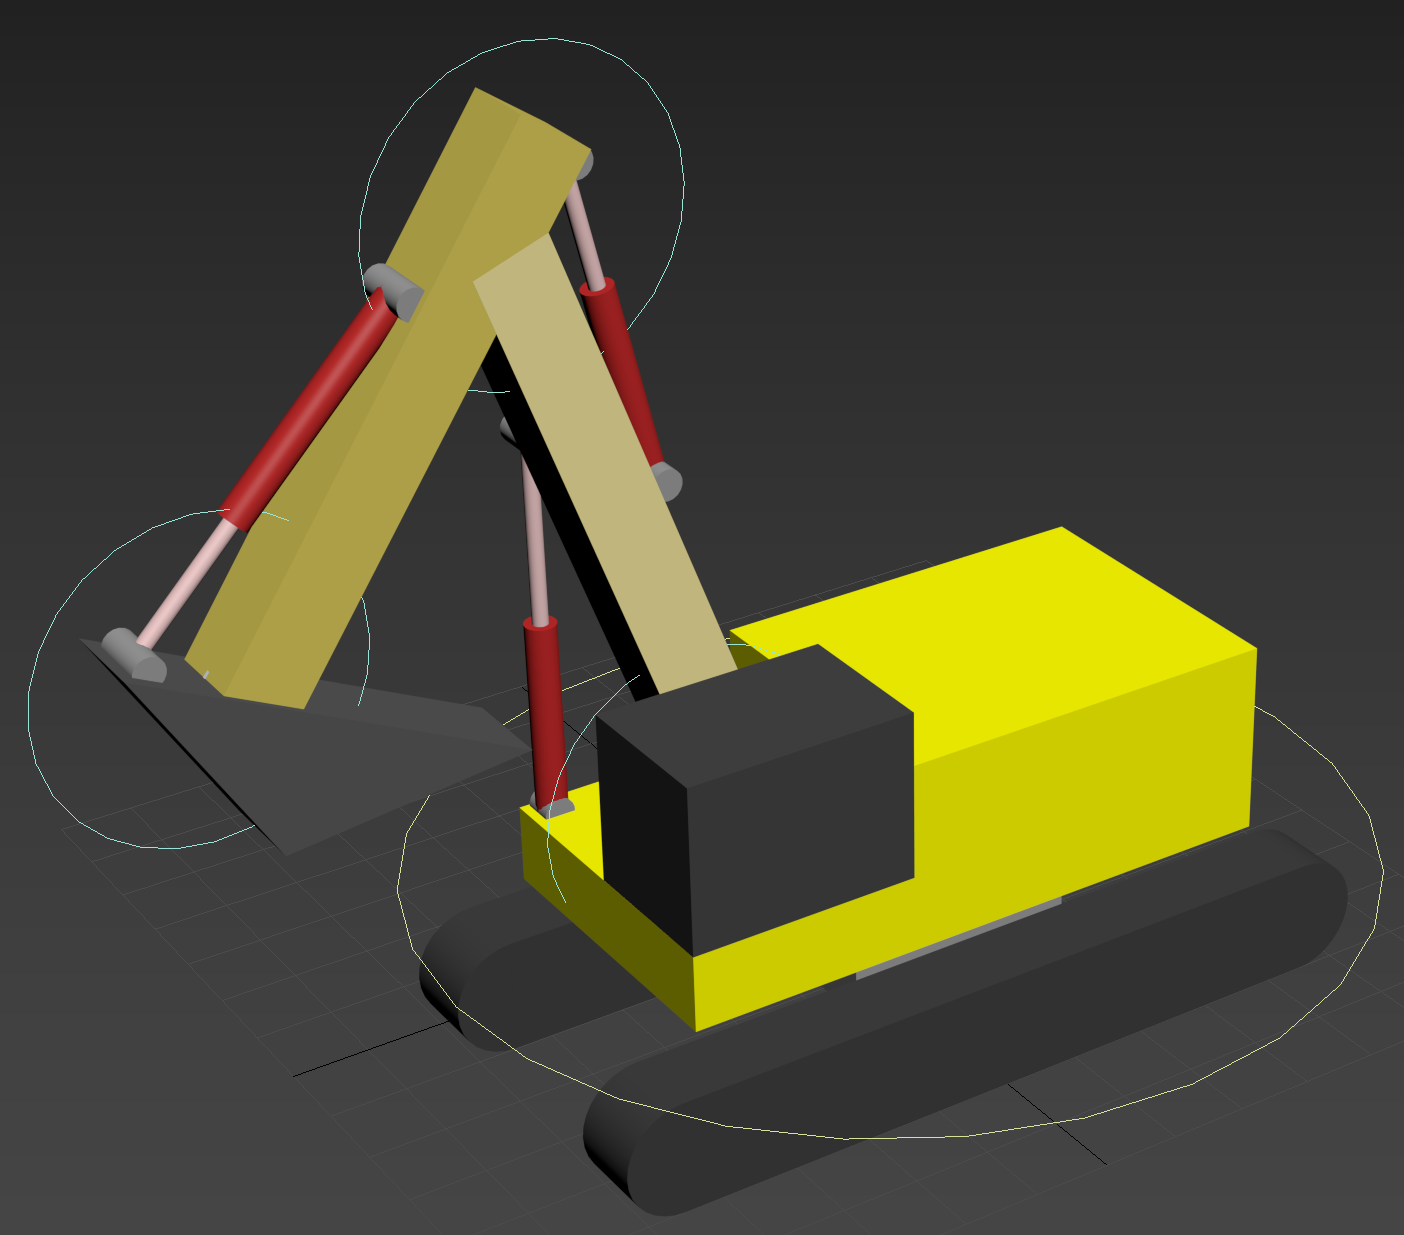
\includegraphics[width=0.5\textwidth]{imagenes/excavadora.png}
   \caption{Modelo final de la excavadora.}
\end{figure}

En las siguientes secciones explicaré el proceso de creación del modelo:
\section{Composición de la excavadora}

Voy a dividir cada una de las partes en subsecciones a continuación:

\subsection{Oruga}

La oruga la he modelado utilizando un cubo alargado y dos cilindros en los extremos con el mismo radio que la altura de los cubos, de manera que dé la sensación de oruga.

% foto de la oruga y la composicion (o no)

\subsection{Cabina}

La cabina está formada por 4 cubos: Uno primero para realizar la base sobre la que va a girar la propia cabina, otro donde se pondrá lo demás, uno atrás para hacer el compartimento del motor y uno último para hacer la ventana del conductor.

% foto de la forma final

\subsection{Brazo}

El brazo lo he realizado utilizando dos cubos alargados para cada extremidad. Mientras que la pala la he modelado utilizando un cilindro de base triangular escalado en uno de sus lados, para que sea más similar a la realidad.

% foto del brazo

Cabe destacar que he añadido pistones hidráulicos a las secciones del brazo para que sea más realista. Los pistones se modelan de la misma forma que en el seminario, con la única diferencia que los puntos de apoyo tienen un \textit{Link Position} para que se mantengan siempre pegados al brazo.

% foto del pistón
\section{Posición de reposo}

La posición de reposo de la excavadora es la siguiente:

% foto de la posición de la excavadora

Para realizarlo, he seleccionado todo el modelo, salvo los \textit{sliders} y los pistones, ya que la posición de reposo eliminaba el \textit{LookAt Constraint} de los pistones.

\bigskip

Cabe destacar que se podría haber hecho la posición de reposo a los pistones también, añadiendo el controlador de nuevo, pero no he llegado a conseguir que funcione del todo bien, por lo que lo he dejado así.

\bigskip

La única desventaja que tiene esta configuración es que al elegir \textit{Transform To Zero}, aparecerán varias veces el siguiente error:

% foto del error

Esto es debido a que los pistones no tienen posición congelada.
\section{Restricciones}

Voy a dividir esta sección en varias subsecciones:

\subsection{Pistones}

Los pistones tienen las siguientes restricciones:

% fotos de las restricciones
\begin{figure}[H]
    \centering
    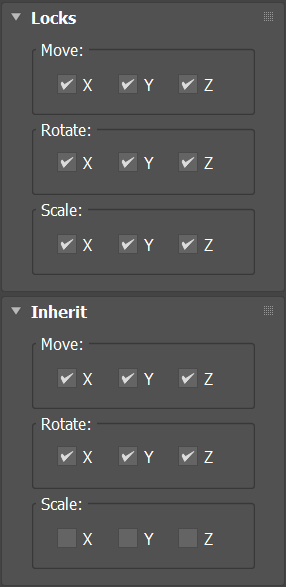
\includegraphics[width=0.2\textwidth]{imagenes/pistonlock.png}
    \caption{Restricciones aplicadas a los pistones.}
 \end{figure}

Como se puede ver, he bloqueado cualquier posibilidad de transformación, ya que el pistón es un objeto que debe seguir el movimiento de los demás. Además, he prohibido la herencia de escalado, ya que en el caso del pistón con la pala, se daba el caso de que se deformaba.

\bigskip

Asimismo, los cilindros que se estiran y comprimen (los que no hacen de soporte) tienen un \textit{LookAt Constraint} que se apuntan mutuamente para seguir el movimiento de manera realista.

\bigskip

Por último, los puntos de apoyo de los pistones tienen un \textit{Link Position} con la unión en el hueso que le corresponde.

\newpage

\subsection{Controladores}

Los controladores del brazo tienen las siguientes restricciones:

% foto de las restricciones
\begin{figure}[H]
    \centering
    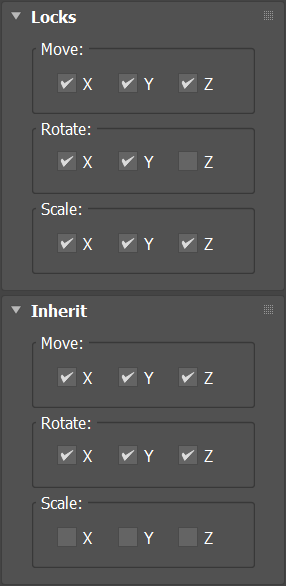
\includegraphics[width=0.2\textwidth]{imagenes/controladorverticallock.png}
    \caption{Restricciones aplicadas a los controladores.}
 \end{figure}

Así se prohíbe realizar movimientos del brazo no permitidos, como girar de izquierda a derecha. Además, las restricciones aplicadas al controlador que gira toda la excavadora prohíben giros incorrectos sobre cualquier otro eje que no sea el eje Z.

\subsection{Resto de figuras}

El resto de figuras tienen bloqueados todas las transformaciones, ya que son los controladores los que se encargan de mover los huesos de la grúa.
\section{Capas}

He dividido los componentes de la grúa en 3 capas:

\begin{itemize}
    \item \textbf{Controladores: }Esta capa almacena los \textit{sliders} que controlan el movimiento de la excavadora y los controladores de los huesos.
    
    % foto de eso

    \item \textbf{Esqueleto: }No habría sido necesario en esta figura, pero he decidí usarlos en una etapa muy temprana y ya es muy complicado cambiarlo.
    
    Los huesos de la excavadora son:


    % foto de los huesos

    Como se puede ver, tiene un hueso debajo que es el que se encarga de mover toda la cabina y el brazo. Después, tiene los huesos del propio brazo.

    \item \textbf{Modelo: }Esta capa es la utilizada para almacenar el modelo de la excavadora.
    
    % foto de la capa
\end{itemize}

% \bibliographystyle{plainurl} % We choose the "plain" reference style
% \bibliography{bib} % Entries are in the refs.bib file

\end{document}
